\chapter{Numerical results} \label{chap:results}
In this chapter we present some numerical results. The convergence of higher 
order methods applied to the Navier-Stokes equations is tested, first in space, 
then in time. Then another spatial comparison test between the upwind method 
and the TVD methods is performed using a channel flow. After that the results 
from the backward facing step test using the RANS equations are shown and 
compared to those from the CFL3D code \cite{web:nasa}. Next, a turbulent 
channel flow with two small cavities is studied and at last a coupled free-flow 
and porous-medium flow problem is analysed, varying the permeability of the 
porous-medium.\\
In all the tests the gravity has been neglected.
%
\section{Navier-Stokes tests}
\subsection{Space convergence} \label{subsec:conv}
We want to test the spatial convergence order of the $L^2$-error of the 
solution of the Navier-Stokes equations, comparing the results obtained with 
the upwind method \eqref{eq:upwind} and the TVD methods described in 
Subsection~\ref{subsec:tvd}.\\
We consider a steady version of the 
equations~\eqref{eq:nsmass}--\eqref{eq:nsmom}:
\begin{align}
	\label{eq:nssteadymass} \nabla \cdot \mathbf{v} -h = 0&\\
	\label{eq:nssteadymom} \nabla \cdot (\mathbf{v} \mathbf{v}^\mathrm{T}) - 
	\nabla \cdot (\nu \nabla \mathbf{v}) + \frac{1}{\varrho}\nabla p  
	-\mathbf{f} = \mathbf{0}&
\end{align}
We neglect the gravity, but we take into account two possible source terms 
$h$ and $\mathbf{f}$. Moreover, for the sake of simplicity, we consider here 
all the quantities appearing in the equations to be non-dimensional.
%
\subsubsection{Sin-Cos test}
Let us solve the equations~\eqref{eq:nssteadymass}--\eqref{eq:nssteadymom} over 
a two-dimensional unit domain $\Omega=(0,1)^2$, with the following source terms:
\begin{align}
	h &= 0,\\
	\mathbf{f} &= [-2\nu \cos(x) \sin(y), \; 2\nu \cos(y) \sin(x)]^\mathrm{T},
\end{align}
so that, choosing $\varrho=1$, the analytical solution, depicted in 
Figure~\ref{fig:sincosexact}, is given by
\begin{align}
\label{eq:uexsin}	u_\text{ex}(x,y) &= -\cos(x)\sin(y)\\
	v_\text{ex}(x,y) &= \sin(x)\cos(y)\\
\label{eq:pexsin}	p_\text{ex}(x,y) &= -\frac{\cos(2x)+\sin(2y)}{4}
\end{align}
Dirichlet boundary conditions for the velocity are applied on the whole 
boundary $\partial \Omega$ using the exact solution. Because of this choice, 
the pressure appears in the problem only in the momentum equation 
\eqref{eq:nssteadymom}, under the sign of gradient. Thus in the numerical 
solution it would be defined up to a constant, so we fix its value at one point 
in the domain in order to match the exact solution \eqref{eq:pexsin}.
\begin{figure}
	\centering
	\subfloat{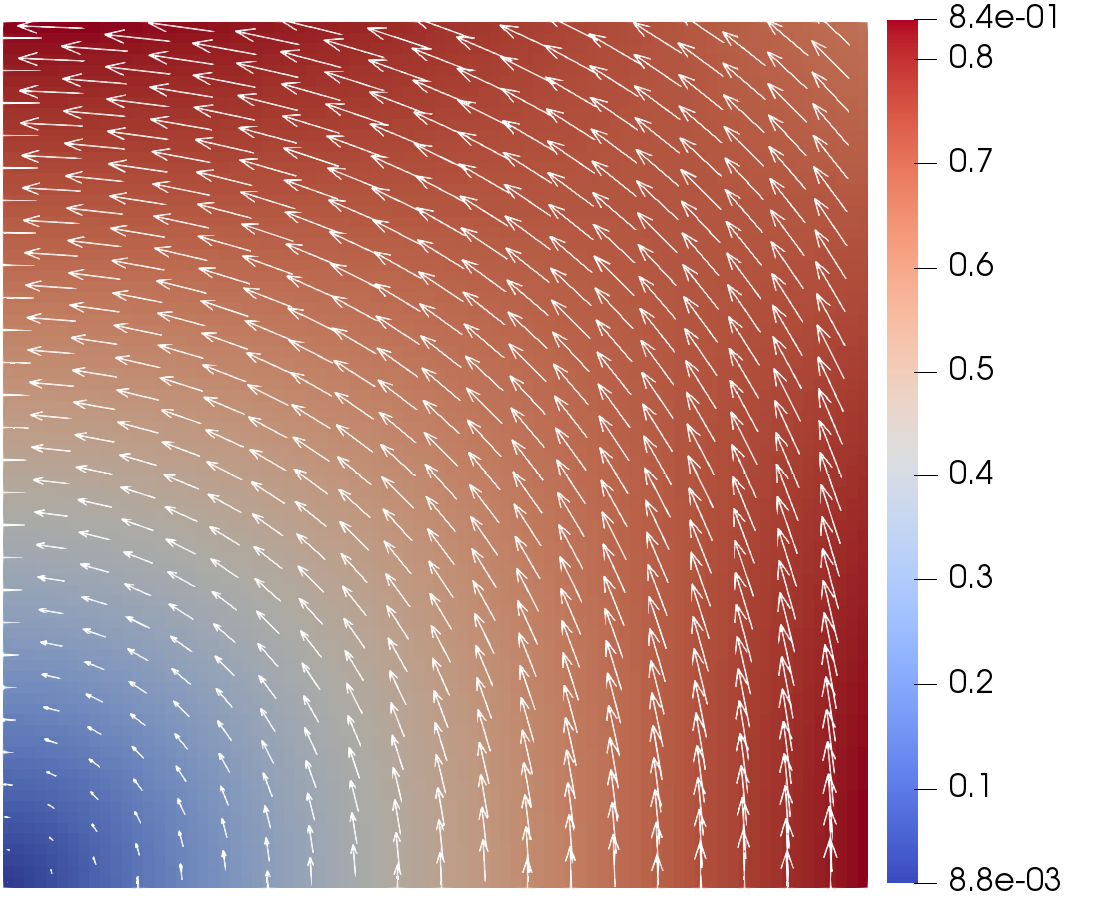
\includegraphics[width=0.5\textwidth]{sincos_exact_v_report.png}}
	\subfloat{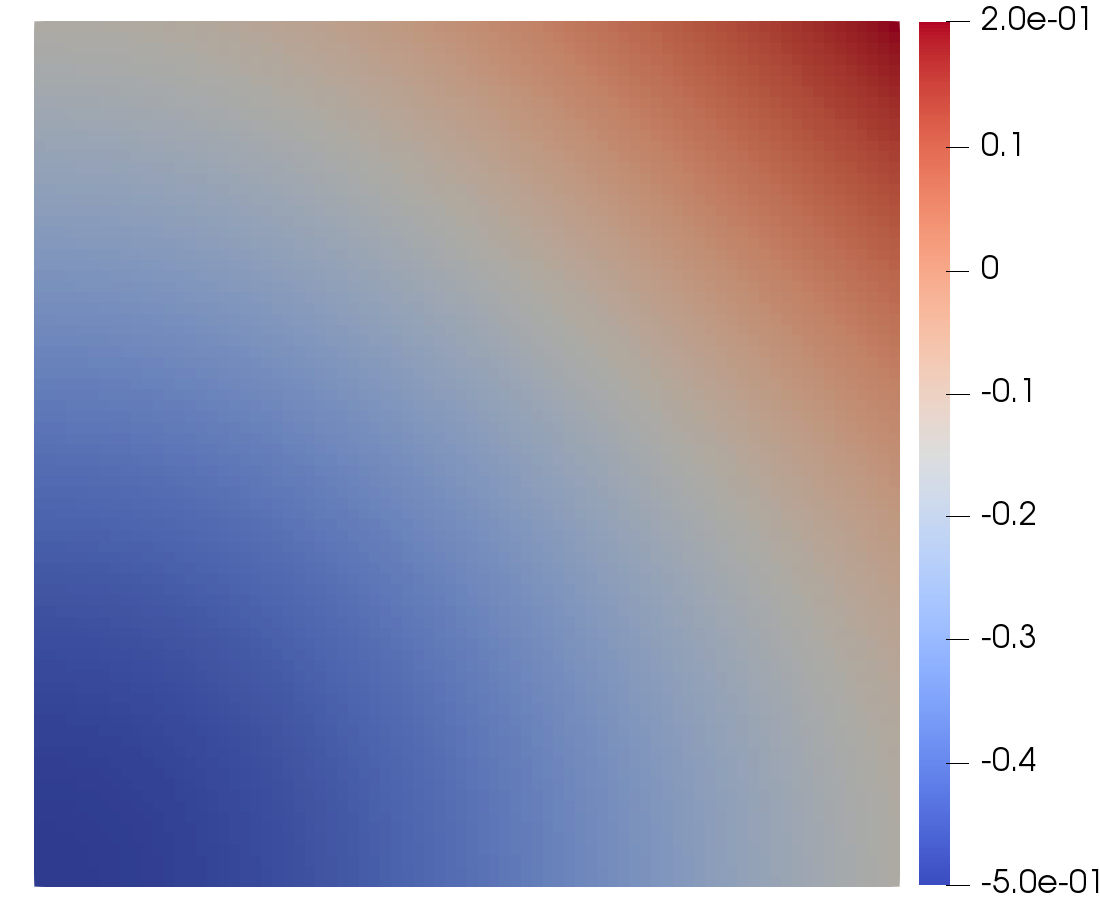
\includegraphics[width=0.5\textwidth]{sincos_exact_p_report.png}}
	\caption[Exact solution of the Sin-Cos test]{Exact solution of the Sin-Cos 
	test \eqref{eq:uexsin}--\eqref{eq:pexsin}. On the left the magnitude of the 
	velocity field, on the right the 
	pressure field.}
	\label{fig:sincosexact}
\end{figure}

The problem is solved over a sequence of five uniform grids, starting from 
$\num{4x4}$ cells and each time halving their size. Both the cases of $\nu=1$ 
and $\nu=\num{e-3}$ are considered, that correspond to $Re=1$ and $Re=\num{e3}$ 
respectively. In Figure~\ref{fig:sin_err} the errors computed are reported 
depending on the square root of the number of cells, while in 
Tables~\ref{tab:sin_lre}--\ref{tab:sin_hre} we can compare directly the 
convergence orders for the different differencing schemes.
\begin{figure}
	\centering
	\subfloat[Upwind, $Re = 1$]{
		% This file was created by matlab2tikz.
%
\definecolor{mycolor1}{rgb}{0.00000,0.44700,0.74100}%
\definecolor{mycolor2}{rgb}{0.85000,0.32500,0.09800}%
\definecolor{mycolor3}{rgb}{0.92900,0.69400,0.12500}%
%
\begin{tikzpicture}

\begin{axis}[%
width=0.951\figwidth,
height=0.75\figwidth,
at={(0\figwidth,0\figwidth)},
scale only axis,
xmode=log,
xmin=4,
xmax=100,
xminorticks=true,
ymode=log,
ymin=1e-05,
ymax=0.1,
yminorticks=true,
axis background/.style={fill=white},
legend style={at={(0.97,0.97)}, anchor=north east, legend cell align=left, align=left, draw=white!15!black}
]
\addplot [color=mycolor1, mark=x, mark options={solid, mycolor1}]
  table[row sep=crcr]{%
4	0.0377253281\\
8	0.016292839\\
16	0.00647505826\\
32	0.00277859939\\
64	0.00131783073\\
};
\addlegendentry{$p$}

\addplot [color=mycolor2, mark=x, mark options={solid, mycolor2}]
  table[row sep=crcr]{%
4	0.00100309389\\
8	0.000409725552\\
16	0.000134946447\\
32	5.06672786e-05\\
64	2.29407924e-05\\
};
\addlegendentry{$u$}

\addplot [color=mycolor3, mark=x, mark options={solid, mycolor3}]
  table[row sep=crcr]{%
4	0.000631316968\\
8	0.000278812074\\
16	0.00010907144\\
32	4.76177485e-05\\
64	2.28652417e-05\\
};
\addlegendentry{$v$}

\addplot [color=white!70!black, forget plot]
  table[row sep=crcr]{%
4	0.00025\\
100	1e-05\\
};
\addplot [color=white!70!black, forget plot]
  table[row sep=crcr]
	\subfloat[Upwind, $Re = \num{e3}$]{
		% This file was created by matlab2tikz.
%
\definecolor{mycolor1}{rgb}{0.00000,0.44700,0.74100}%
\definecolor{mycolor2}{rgb}{0.85000,0.32500,0.09800}%
\definecolor{mycolor3}{rgb}{0.92900,0.69400,0.12500}%
%
\begin{tikzpicture}

\begin{axis}[%
width=0.951\figwidth,
height=0.75\figwidth,
at={(0\figwidth,0\figwidth)},
scale only axis,
xmode=log,
xmin=4,
xmax=100,
xminorticks=true,
ymode=log,
ymin=0.00266295649,
ymax=0.1,
yminorticks=true,
axis background/.style={fill=white},
legend style={at={(0.97,0.97)}, anchor=north east, legend cell align=left, align=left}
]
\addplot [color=mycolor1, mark=x, mark options={solid, mycolor1}]
  table[row sep=crcr]{%
4	0.0596083589\\
8	0.0364982308\\
16	0.0196434526\\
32	0.00962257784\\
64	0.00434161729\\
};
\addlegendentry{$p$}

\addplot [color=mycolor2, mark=x, mark options={solid, mycolor2}]
  table[row sep=crcr]{%
4	0.0339372138\\
8	0.0206751686\\
16	0.011131246\\
32	0.00559430586\\
64	0.00266295649\\
};
\addlegendentry{$u$}

\addplot [color=mycolor3, mark=x, mark options={solid, mycolor3}]
  table[row sep=crcr]{%
4	0.0347600515\\
8	0.0213374017\\
16	0.0114856296\\
32	0.00577467407\\
64	0.00275450966\\
};
\addlegendentry{$v$}

\addplot [color=white!70!black, forget plot]
  table[row sep=crcr]{%
4	0.06657391225\\
100	0.00266295649\\
};
\addplot [color=white!70!black, forget plot]
  table[row sep=crcr]\\
	\subfloat[Min-Mod, $Re = 1$]{
		% This file was created by matlab2tikz.
%
\definecolor{mycolor1}{rgb}{0.00000,0.44700,0.74100}%
\definecolor{mycolor2}{rgb}{0.85000,0.32500,0.09800}%
\definecolor{mycolor3}{rgb}{0.92900,0.69400,0.12500}%
%
\begin{tikzpicture}

\begin{axis}[%
width=0.951\figwidth,
height=0.75\figwidth,
at={(0\figwidth,0\figwidth)},
scale only axis,
xmode=log,
xmin=4,
xmax=100,
xminorticks=true,
ymode=log,
ymin=1e-05,
ymax=0.1,
yminorticks=true,
axis background/.style={fill=white},
legend style={at={(0.97,0.97)}, anchor=north east, legend cell align=left, align=left}
]
\addplot [color=mycolor1, mark=x, mark options={solid, mycolor1}]
  table[row sep=crcr]{%
4	0.0201961443\\
8	0.00658170291\\
16	0.00181646151\\
32	0.000558641084\\
64	0.000188245776\\
};
\addlegendentry{$p$}

\addplot [color=mycolor2, mark=x, mark options={solid, mycolor2}]
  table[row sep=crcr]{%
4	0.00148598782\\
8	0.00053497283\\
16	0.000150385476\\
32	3.95894587e-05\\
64	1.01636468e-05\\
};
\addlegendentry{$u$}

\addplot [color=mycolor3, mark=x, mark options={solid, mycolor3}]
  table[row sep=crcr]{%
4	0.00119526142\\
8	0.00045470553\\
16	0.000138075359\\
32	3.80865907e-05\\
64	1.00057526e-05\\
};
\addlegendentry{$v$}

\addplot [color=white!70!black, forget plot]
  table[row sep=crcr]{%
4	0.00025\\
100	1e-05\\
};
\addplot [color=white!70!black, forget plot]
  table[row sep=crcr]
	\subfloat[Min-Mod, $Re = \num{e3}$]{
		% This file was created by matlab2tikz.
%
\definecolor{mycolor1}{rgb}{0.00000,0.44700,0.74100}%
\definecolor{mycolor2}{rgb}{0.85000,0.32500,0.09800}%
\definecolor{mycolor3}{rgb}{0.92900,0.69400,0.12500}%
%
\begin{tikzpicture}

\begin{axis}[%
width=0.951\figwidth,
height=0.75\figwidth,
at={(0\figwidth,0\figwidth)},
scale only axis,
xmode=log,
xmin=4,
xmax=100,
xminorticks=true,
ymode=log,
ymin=0.0001,
ymax=0.0206930353,
yminorticks=true,
axis background/.style={fill=white},
legend style={at={(0.97,0.97)}, anchor=north east, legend cell align=left, align=left}
]
\addplot [color=mycolor1, mark=x, mark options={solid, mycolor1}]
  table[row sep=crcr]{%
4	0.0206930353\\
8	0.0102262223\\
16	0.00364544433\\
32	0.000812298263\\
64	0.000257143964\\
};
\addlegendentry{$p$}

\addplot [color=mycolor2, mark=x, mark options={solid, mycolor2}]
  table[row sep=crcr]{%
4	0.0130268788\\
8	0.00605072242\\
16	0.00243635311\\
32	0.000918041806\\
64	0.000338134479\\
};
\addlegendentry{$u$}

\addplot [color=mycolor3, mark=x, mark options={solid, mycolor3}]
  table[row sep=crcr]{%
4	0.0129926934\\
8	0.00750558766\\
16	0.0037160882\\
32	0.00148526754\\
64	0.000512917943\\
};
\addlegendentry{$v$}

\addplot [color=white!70!black, forget plot]
  table[row sep=crcr]{%
4	0.0025\\
100	0.0001\\
};
\addplot [color=white!70!black, forget plot]
  table[row sep=crcr]\\
	\subfloat[Van Leer, $Re = 1$]{
		% This file was created by matlab2tikz.
%
\definecolor{mycolor1}{rgb}{0.00000,0.44700,0.74100}%
\definecolor{mycolor2}{rgb}{0.85000,0.32500,0.09800}%
\definecolor{mycolor3}{rgb}{0.92900,0.69400,0.12500}%
%
\begin{tikzpicture}

\begin{axis}[%
width=0.951\figwidth,
height=0.75\figwidth,
at={(0\figwidth,0\figwidth)},
scale only axis,
xmode=log,
xmin=4,
xmax=100,
xminorticks=true,
ymode=log,
ymin=8.63199669e-06,
ymax=0.1,
yminorticks=true,
axis background/.style={fill=white},
legend style={at={(0.03,0.03)}, anchor=south west, legend cell align=left, align=left, draw=white!15!black}
]
\addplot [color=mycolor1, mark=x, mark options={solid, mycolor1}]
  table[row sep=crcr]{%
4	0.017335487\\
8	0.0062618753\\
16	0.00193371119\\
32	0.000605597659\\
64	0.000196206927\\
};
\addlegendentry{$p$}

\addplot [color=mycolor2, mark=x, mark options={solid, mycolor2}]
  table[row sep=crcr]{%
4	0.00136409678\\
8	0.000476275877\\
16	0.000131606902\\
32	3.41242821e-05\\
64	8.66824542e-06\\
};
\addlegendentry{$u$}

\addplot [color=mycolor3, mark=x, mark options={solid, mycolor3}]
  table[row sep=crcr]{%
4	0.00114596769\\
8	0.000417513208\\
16	0.000122988533\\
32	3.32359157e-05\\
64	8.63199669e-06\\
};
\addlegendentry{$v$}

\addplot [color=white!70!black, forget plot]
  table[row sep=crcr]{%
4	0.00021579991725\\
100	8.63199669e-06\\
};
\addplot [color=white!70!black, forget plot]
  table[row sep=crcr]
	\subfloat[Van Leer, $Re = \num{e3}$]{
		% This file was created by matlab2tikz.
%
\definecolor{mycolor1}{rgb}{0.00000,0.44700,0.74100}%
\definecolor{mycolor2}{rgb}{0.85000,0.32500,0.09800}%
\definecolor{mycolor3}{rgb}{0.92900,0.69400,0.12500}%
%
\begin{tikzpicture}

\begin{axis}[%
width=0.951\figwidth,
height=0.75\figwidth,
at={(0\figwidth,0\figwidth)},
scale only axis,
xmode=log,
xmin=4,
xmax=100,
xminorticks=true,
ymode=log,
ymin=0.0001,
ymax=0.01454297,
yminorticks=true,
axis background/.style={fill=white},
legend style={at={(0.97,0.97)}, anchor=north east, legend cell align=left, align=left}
]
\addplot [color=white!70!black, forget plot, line width=0.75pt]
  table[row sep=crcr]{%
4	0.0025\\
100	0.0001\\
};
\addplot [color=white!70!black, forget plot, line width=0.75pt]
  table[row sep=crcr]{%
4	0.0625\\
100	0.0001\\
};
\addplot [color=mycolor1, mark=x, mark options={solid, mycolor1}, line width=0.75pt]
  table[row sep=crcr]{%
4	0.01454297\\
8	0.00653869074\\
16	0.00224775854\\
32	0.0005196908\\
64	0.000249600967\\
};
\addlegendentry{$p$}

\addplot [color=mycolor2, mark=x, mark options={solid, mycolor2}, line width=0.75pt]
  table[row sep=crcr]{%
4	0.0107200353\\
8	0.00466675248\\
16	0.00177426299\\
32	0.000645881865\\
64	0.000238530337\\
};
\addlegendentry{$u$}

\addplot [color=mycolor3, mark=x, mark options={solid, mycolor3}, line width=0.75pt]
  table[row sep=crcr]
	\caption[$L^2$-errors for the Sin-Cos problem]{$L^2$-errors for the Sin-Cos 
	problem depending on the square root of the number of cells in the grid. 
	The grey lines are the reference lines for the first-order and second-order 
	convergence.}
	\label{fig:sin_err}
\end{figure}
\begin{table}
	\centering
	\[
	\begin{array}{c|ccc}
	\toprule
	& \text{Upwind} & \text{Min-Mod} & \text{Van Leer} \\ 
	\midrule
	p & 1.008 & 1.569 & 1.626\\
	v_x & 1.143 & 1.962 & 1.977\\
	v_y & 1.058 & 1.928 & 1.945\\
	\bottomrule
	\end{array}
	\]
	\caption[Convergence orders with $Re = 1$ for the Sin-Cos 
	problem]{Convergence orders with $Re = 1$ for the Sin-Cos problem. They are 
	computed considering the last two refinements of the grid.}
	\label{tab:sin_lre}
	\[
	\begin{array}{c|ccc}
	\toprule
	& \text{Upwind} & \text{Min-Mod} & \text{Van Leer} \\ 
	\midrule
	p & 1.148 & 1.659 & 1.058\\
	v_x & 1.071 & 1.441 & 1.437\\
	v_y & 1.068 & 1.533 & 1.560\\
	\bottomrule
	\end{array}
	\]
	\caption[Convergence orders with $Re = \num{e3}$ for the Sin-Cos 
	problem]{Convergence orders with $Re = \num{e3}$ for the Sin-Cos problem. 
	They are computed considering the last two refinements of the grid.}
	\label{tab:sin_hre}
\end{table}

conclusioni

Analogous tests with other analytical solutions are reported in the 
Appendix~\ref{app:conv}.
%
\subsection{Time convergence}
%
\subsection{Rough channel test}
%
\section{RANS tests}
\subsection{Backward facing step}
%The NASA LaRC CFD code CFL3D uses:
%\begin{itemize}
%	\item free-stream turbulence intensity = 0.061\%
%	\item free-stream turbulent viscosity (relative to laminar) = 0.009
%	\item in this case the simulations were \emph{quasi-steady}, i.e. the 
%	solution does not converge readily to a steady state result when a refined 
%	grid is used. However, when run-time accurately, the solution settles down 
%	and becomes reasonably steady (quasi-steady).
%	\item The code is for compressible flows at ``essentially incompressible" 
%	conditions of M=0.128. There may be a very small influence of 
%	compressibility.
%	\item non-dimensional CFD code
%	\item first order turbulence advection in the turbulence transport equations
%	\item Neglects two terms that are zero for incompressible flows
%	\item implicit time advancement (also second order)
%	\item Central differencing in Space? Non lo dice cosa usa, inoltre secondo 
%	me non usa una staggered grid.
%\end{itemize}
\subsection{Cavities reciprocal influence}
%An easy result.
\section{Coupled test}
\subsection{Cavities coupled with the porous-medium}
%A more complex result.